\chapter{Introduction to Momentum Transport}

\section{Viscosity and Demonstrating Momentum Transport}

Viscosity is a measure of a fluid's tendency to resist flow. Generally we represent the viscosity of a fluid by $\mu$. 

Before describing the properties of viscosity and how it changes, let us observe qualitatively how a viscous fluid behaves when we try to make it flow under some forces.

Given below is a simple, illustrative situation:

\begin{figure}[h]
    \centering
    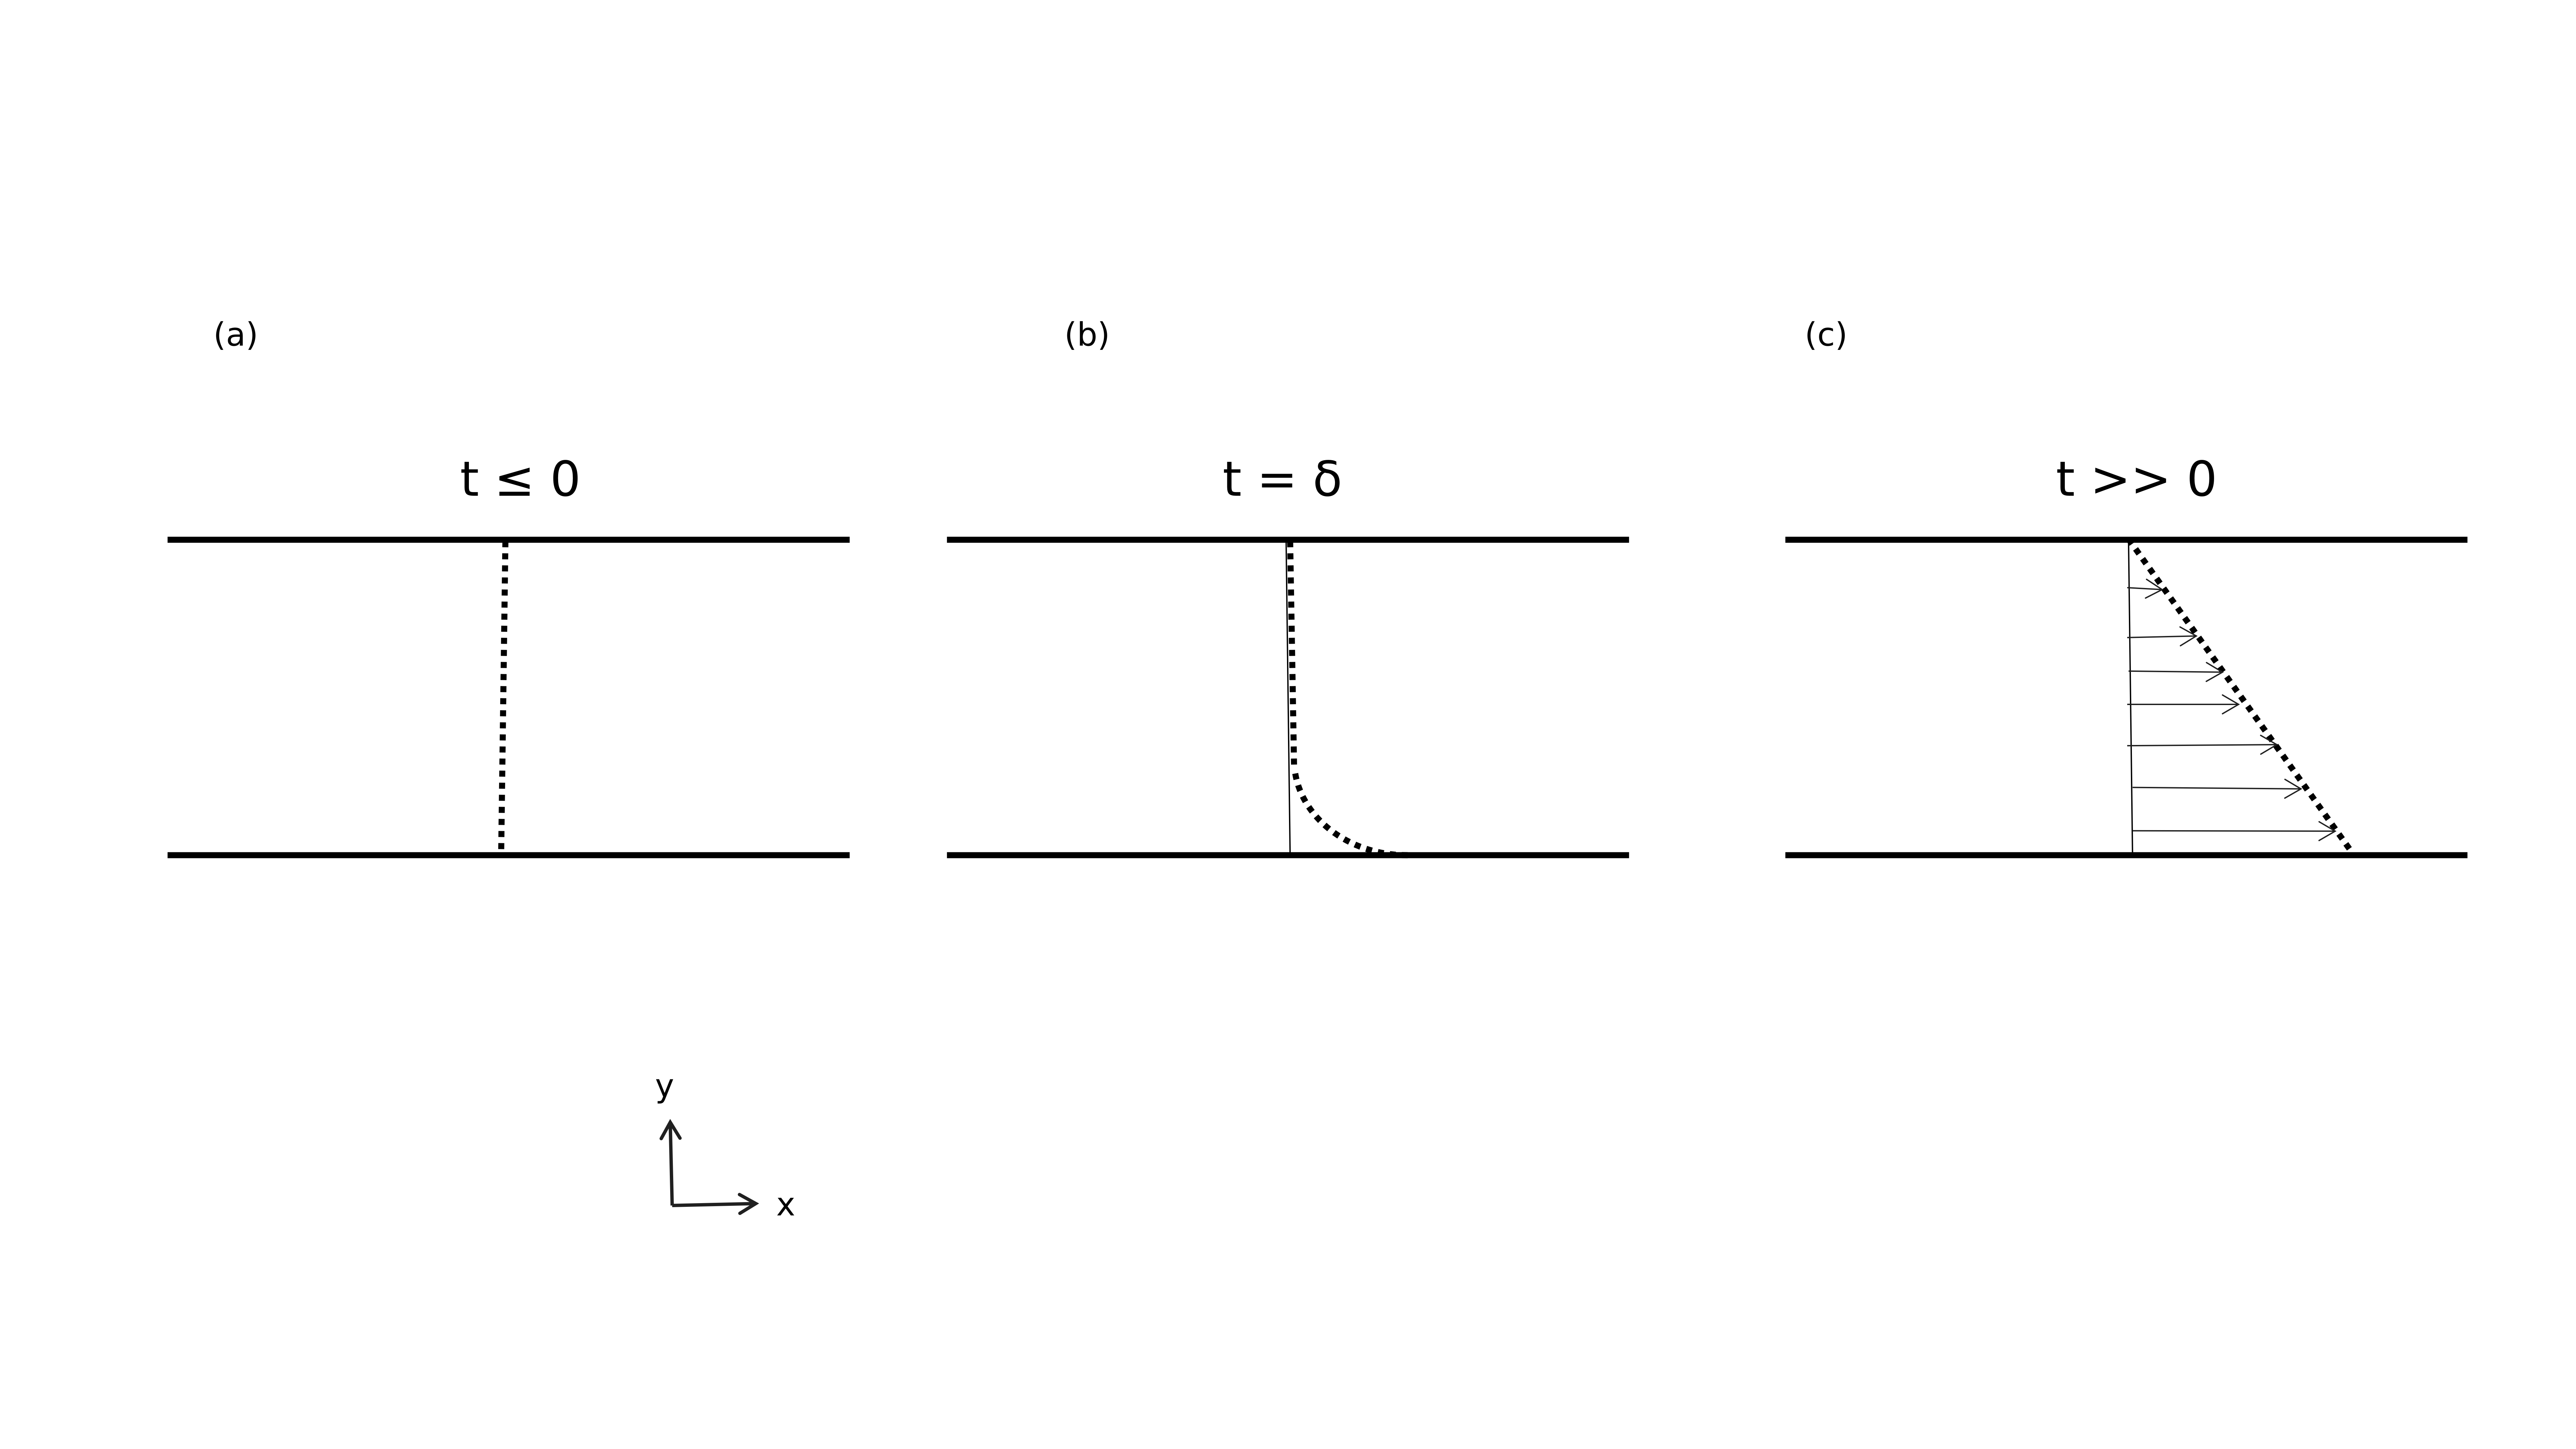
\includegraphics[scale=0.05]{figure1_01}
    \caption{Fluid between 2 plates}
\end{figure}

\begin{itemize}
    \item Consider two parallel plates : one placed at y = 0 and the other placed at y = Y as shown in figure 1.1, with a static fluid between them. Here we assume these plates are basically infinitely long and wide so that the fluid doesn't move. Figure 1.1(a) shows how the fluid velocity is 0 at every point between the two plates. 

    \item Now, let us see what happens when we begin to translate the bottom plate to the right. Assuming there is no slip between the fluid and the plate, i.e. that the fluid that comes into contact with the solid is "stuck" to it. At the molecular scale, this is because we consider adhesive forces of attraction between molecules of the fluid and the solid are stronger than the cohesive forces of attraction among the molecules of the fluid themselves. So when we move the bottom plate, the molecules in contact with it start to move along. Figure 1.1(b) describes a snapshot of the system where the molecules "stuck" to the plate have just started to move but the molecules above them haven't been impacted yet.

    \item Over time, the fluid layers begin to pull each other and due to this, momentum gets imparted along the y direction. Figure 1.1(c) showcases the steady-state velocity profile of the fluid. Again, at the top plate the fluid doesn't move since the molecules are assumed to be "stuck" to the plate. 
\end{itemize}

We began our observation of the transport of momentum by seeing how the fluid molecules in contact with the lower plate are dragged along. But it is important to note that the plate is also being dragged by the fluid! So we have to apply some force F to keep the plate going. How much does the fluid drag the plate?

$$\frac{F}{A} = \mu \frac{V}{Y}$$

This can be extended to looking at the force per unit area that each differential "slice" of fluid experiences:


\begin{empheq}[box=\fbox]{align}
\tau_{yx} = -\mu \frac{dv_{x}}{dy}
\end{empheq}

This is a very important equation and is referred to as Newton's Law of Viscosity.

Some key points to note about Newton's Law of Viscosity:

\begin{itemize}
    \item This equation showcases the transport of the $x$ component of momentum in the y direction.

    \item $\tau_{xy} = F/A$ here refers to the force in $x$ direction per unit area perpendicular to $y$ direction. This quantity is the flux of x-component of momentum in the y direction. 

    \item The law applies to other directions as well. If we consider a pair of \textbf{unequal} directions i, j, we can generalise this and state that $$\tau_{ij} = -\mu \frac{dv_{j}}{di}$$.

    \item If i = j, then we get (for example i = j = x) $$\tau_{xx} = -2 \mu \frac{dv_{x}}{dx}$$.

    \item Here we consider $\mu$ to be invariant of the directions (we don't say $\mu_{xy}$ etc.). This makes an inherent assumption about the isotropy of the fluid, i.e. that the properties of the fluid don't vary in different directions. This is not necessarily true in certain complex fluids and polymer solutions. 
\end{itemize}

Note that it's very easy to see how $\tau$ refers to "momentum flux" by just looking at dimensions. Force is (mass).(acceleration) = (mass).(velocity/time) = (momentum/time) or rate of momentum. Now Force/Area is just flux of momentum, simple!

\textbf{It is very important to remember that $\tau_{yx}$ is the flux of "x-momentum in y direction"}. It is easy to flip the order and make a mistake, so be careful.

\subsection*{Some more points on viscosity}

\begin{itemize}
    \item The dimensions of $\mu$ is (pressure).(time) and hence the SI unit is pascal-second or (Pa)(s). However a more convenient unit for engineering problems is centipoise (cP). Keep in mind that $1 cP = 10^{-3} Pa.s$. Water has a viscosity of about 1 cP at room temperature.

    \item At low densities 
        \SubItem{\textbf{Gases:} Viscosity increases with temperature}
        \SubItem{\textbf{Liquids:} Viscosity decreases with temperature}

    \item Kinematic viscosity can be defined as $$\nu = \frac{\mu}{\rho}$$
\end{itemize}

\section{Mechanisms of Momentum Transport}

\subsection{Vectors and Tensors in Transport}

Some important notation:


\begin{itemize}

    \item \textbf{v} is the velocity vector.

    \item $v_{x}$ is the x component of the velocity vector which is a function: $v_{x} (x, y, z, t)$.

    \item The unit vectors are denoted by \textbf{$\delta_{x}$, $\delta_{y}$, $\delta_{z}$} in x, y, z directions.

    \item Tensors are multilinear objects relating vectors. In the case of fluids, we are mainly concerned with "order 2" tensors, which can be depicted similar to matrices. For example, $\tau$ is an order two tensor whose components are $\tau_{ij}$.

$$\begin{bmatrix}  

    \tau_{xx} & \tau_{xy} & \tau_{xz} \\
    \tau_{yx} & \tau_{yy} & \tau_{yz} \\
    \tau_{zx} & \tau_{zy} & \tau_{zz} \\
    
\end{bmatrix}$$

    \item This is a 9-component tensor. The diagonal components represent normal stresses while other terms are shear stresses.

    \item We can also consider one component out of our tensors: which then becomes a vector. For example if we take the x component of $\tau$, we have $\tau_{x}$ which is a vector.

\end{itemize}


\subsection{Molecular Momentum Transport}

Molecular transport of momentum is the extent of momentum transport that can be attributed to molecular forces. In figure 2, we take a differential fluid element and observe the forces. First let us only consider forces acting in the x-direction, for simplicity. For this, we observe a plane perpendicular to the x-axis (or parallel to the yz plane). For this plane there are 2 forces :

\begin{itemize}
    \item Viscous force $\tau_{x}$ which has three components.

    \item Pressure force $P \delta{x}$. Note again that $\delta_{x}$ is the x-direction unit vector. 
\end{itemize}


\begin{figure}[h]
    \centering
    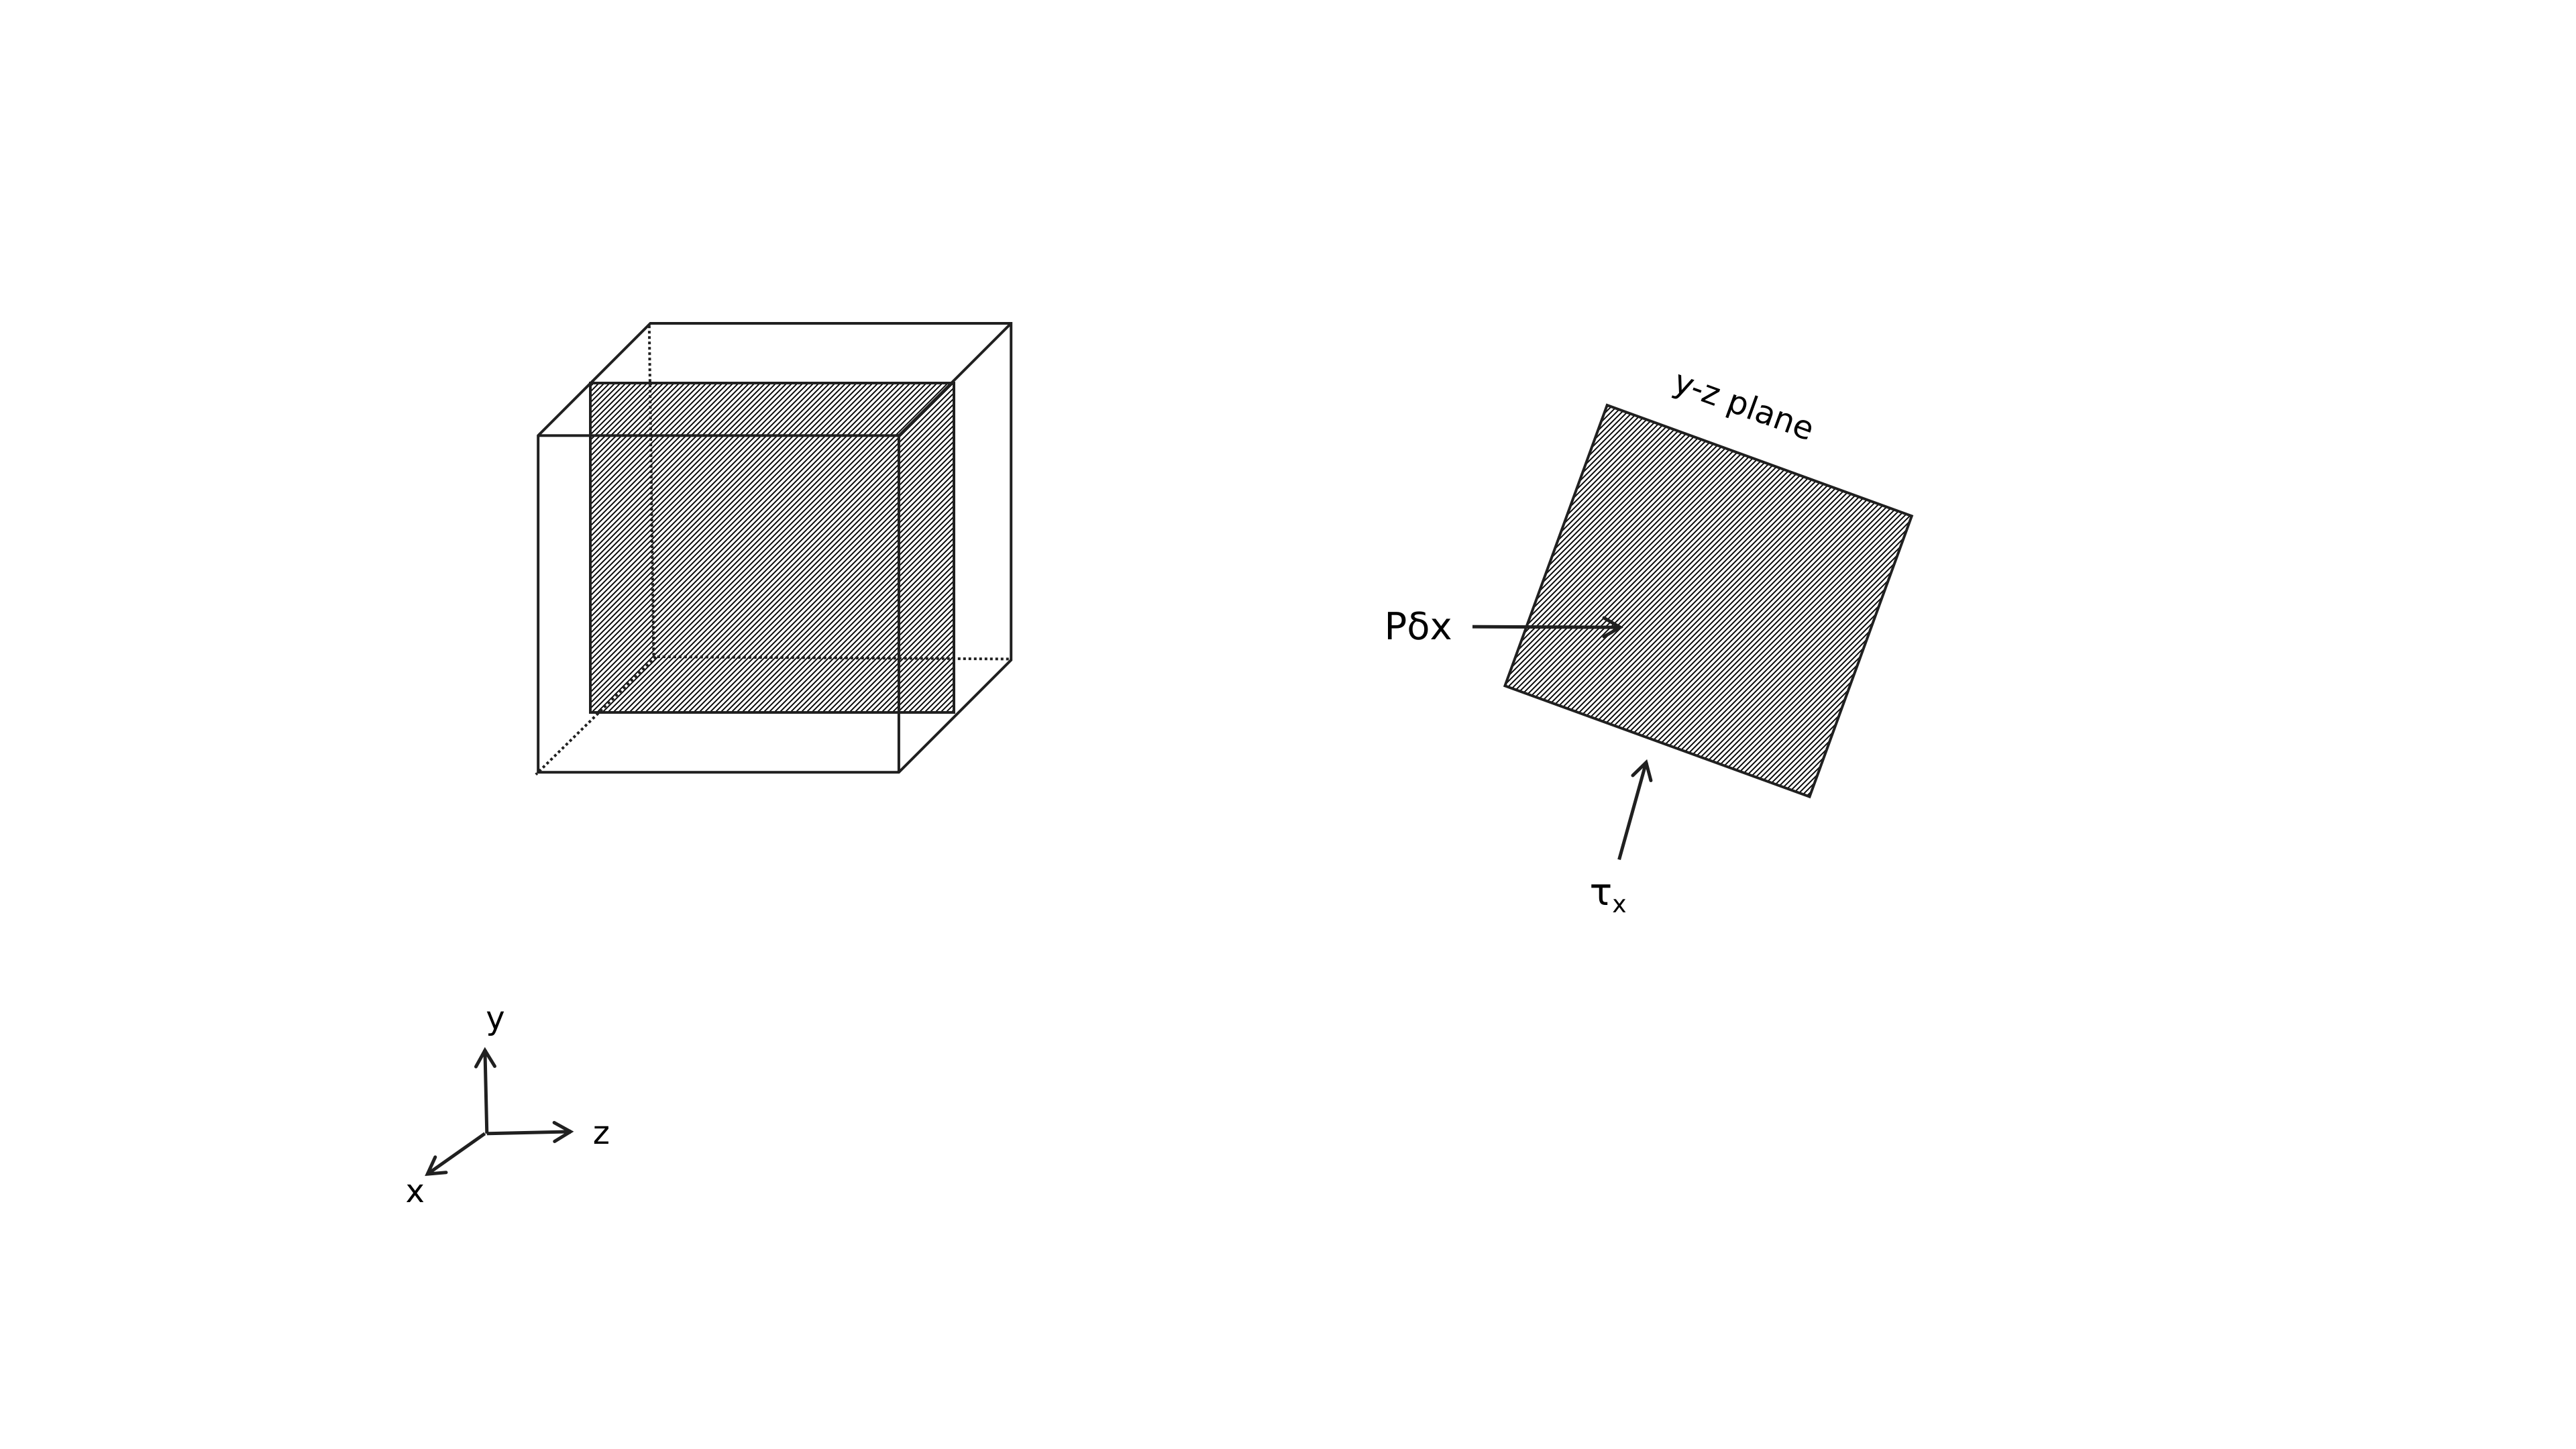
\includegraphics[scale=0.05]{figure2_01}
    \caption{Forces on a fluid element}
\end{figure}


In the absence of a velocity gradient, there are no viscous forces since fluid elements move together but pressure forces still act.

Hence, there are 6 forces tugging this fluid element : 3 pressure forces $P \delta{x}, P \delta{y}, P \delta{z}$ and 3 viscous forces $\tau_{x}, \tau_{y}, \tau_{z}$.

Now, we can define a \textbf{molecular momentum flux} ($\pi$) which gives us the flux of momentum due to molecular forces. We need it to incorporate the pressure term and the viscous term. As described in Figure 2, let us only consider this molecular momentum flux across a plane perpendicular to the x axis.

The viscous terms are easy to incorporate. $\pi_{xx}$ would have the term $\tau_{xx}$, $\pi_{xy}$ would incorporate $\tau_{xy}$ and so on. The pressure term meanwhile only has one direction (x), so we expect it to appear only in the $\pi_{xx}$ expression.

In summary :

$$\pi_{xx} = P + \tau_{xx}$$

$$\pi_{xy} = \tau_{xy}$$

$$\pi_{xz} = \tau_{xz}$$


Similar expressions can be written for $\pi_{y}$ and $\pi_{z}$. For $\pi_{y}$ the pressure term will appear in $\pi_{yy}$ only and for $\pi_{z}$ it'll appear only in $\pi_{zz}$.

If we wanted to condense our expression for $\pi$ into one terse statement, we can write it as such :


\begin{empheq}[box=\fbox]{align}
    \pi_{ij} = P \delta_{ij} + \tau_{ij}
\end{empheq}

Here $\delta_{ij}$ is the Kronecker delta function (which has a value of 1 when i = j and 0 otherwise). \textbf{$\pi_{ij}$ is the flux of j-momentum in the i direction, from a region of less i to greater i.} $\pi$ is again a tensor with the diagonal terms being normal stresses and other components being shear stresses.


\subsection{Convective Momentum Transport}

Apart from molecular forces, momentum can also be transported by bulk flow of fluid. This is called "convective momentum transport". 


\begin{figure}[h]
    \centering
    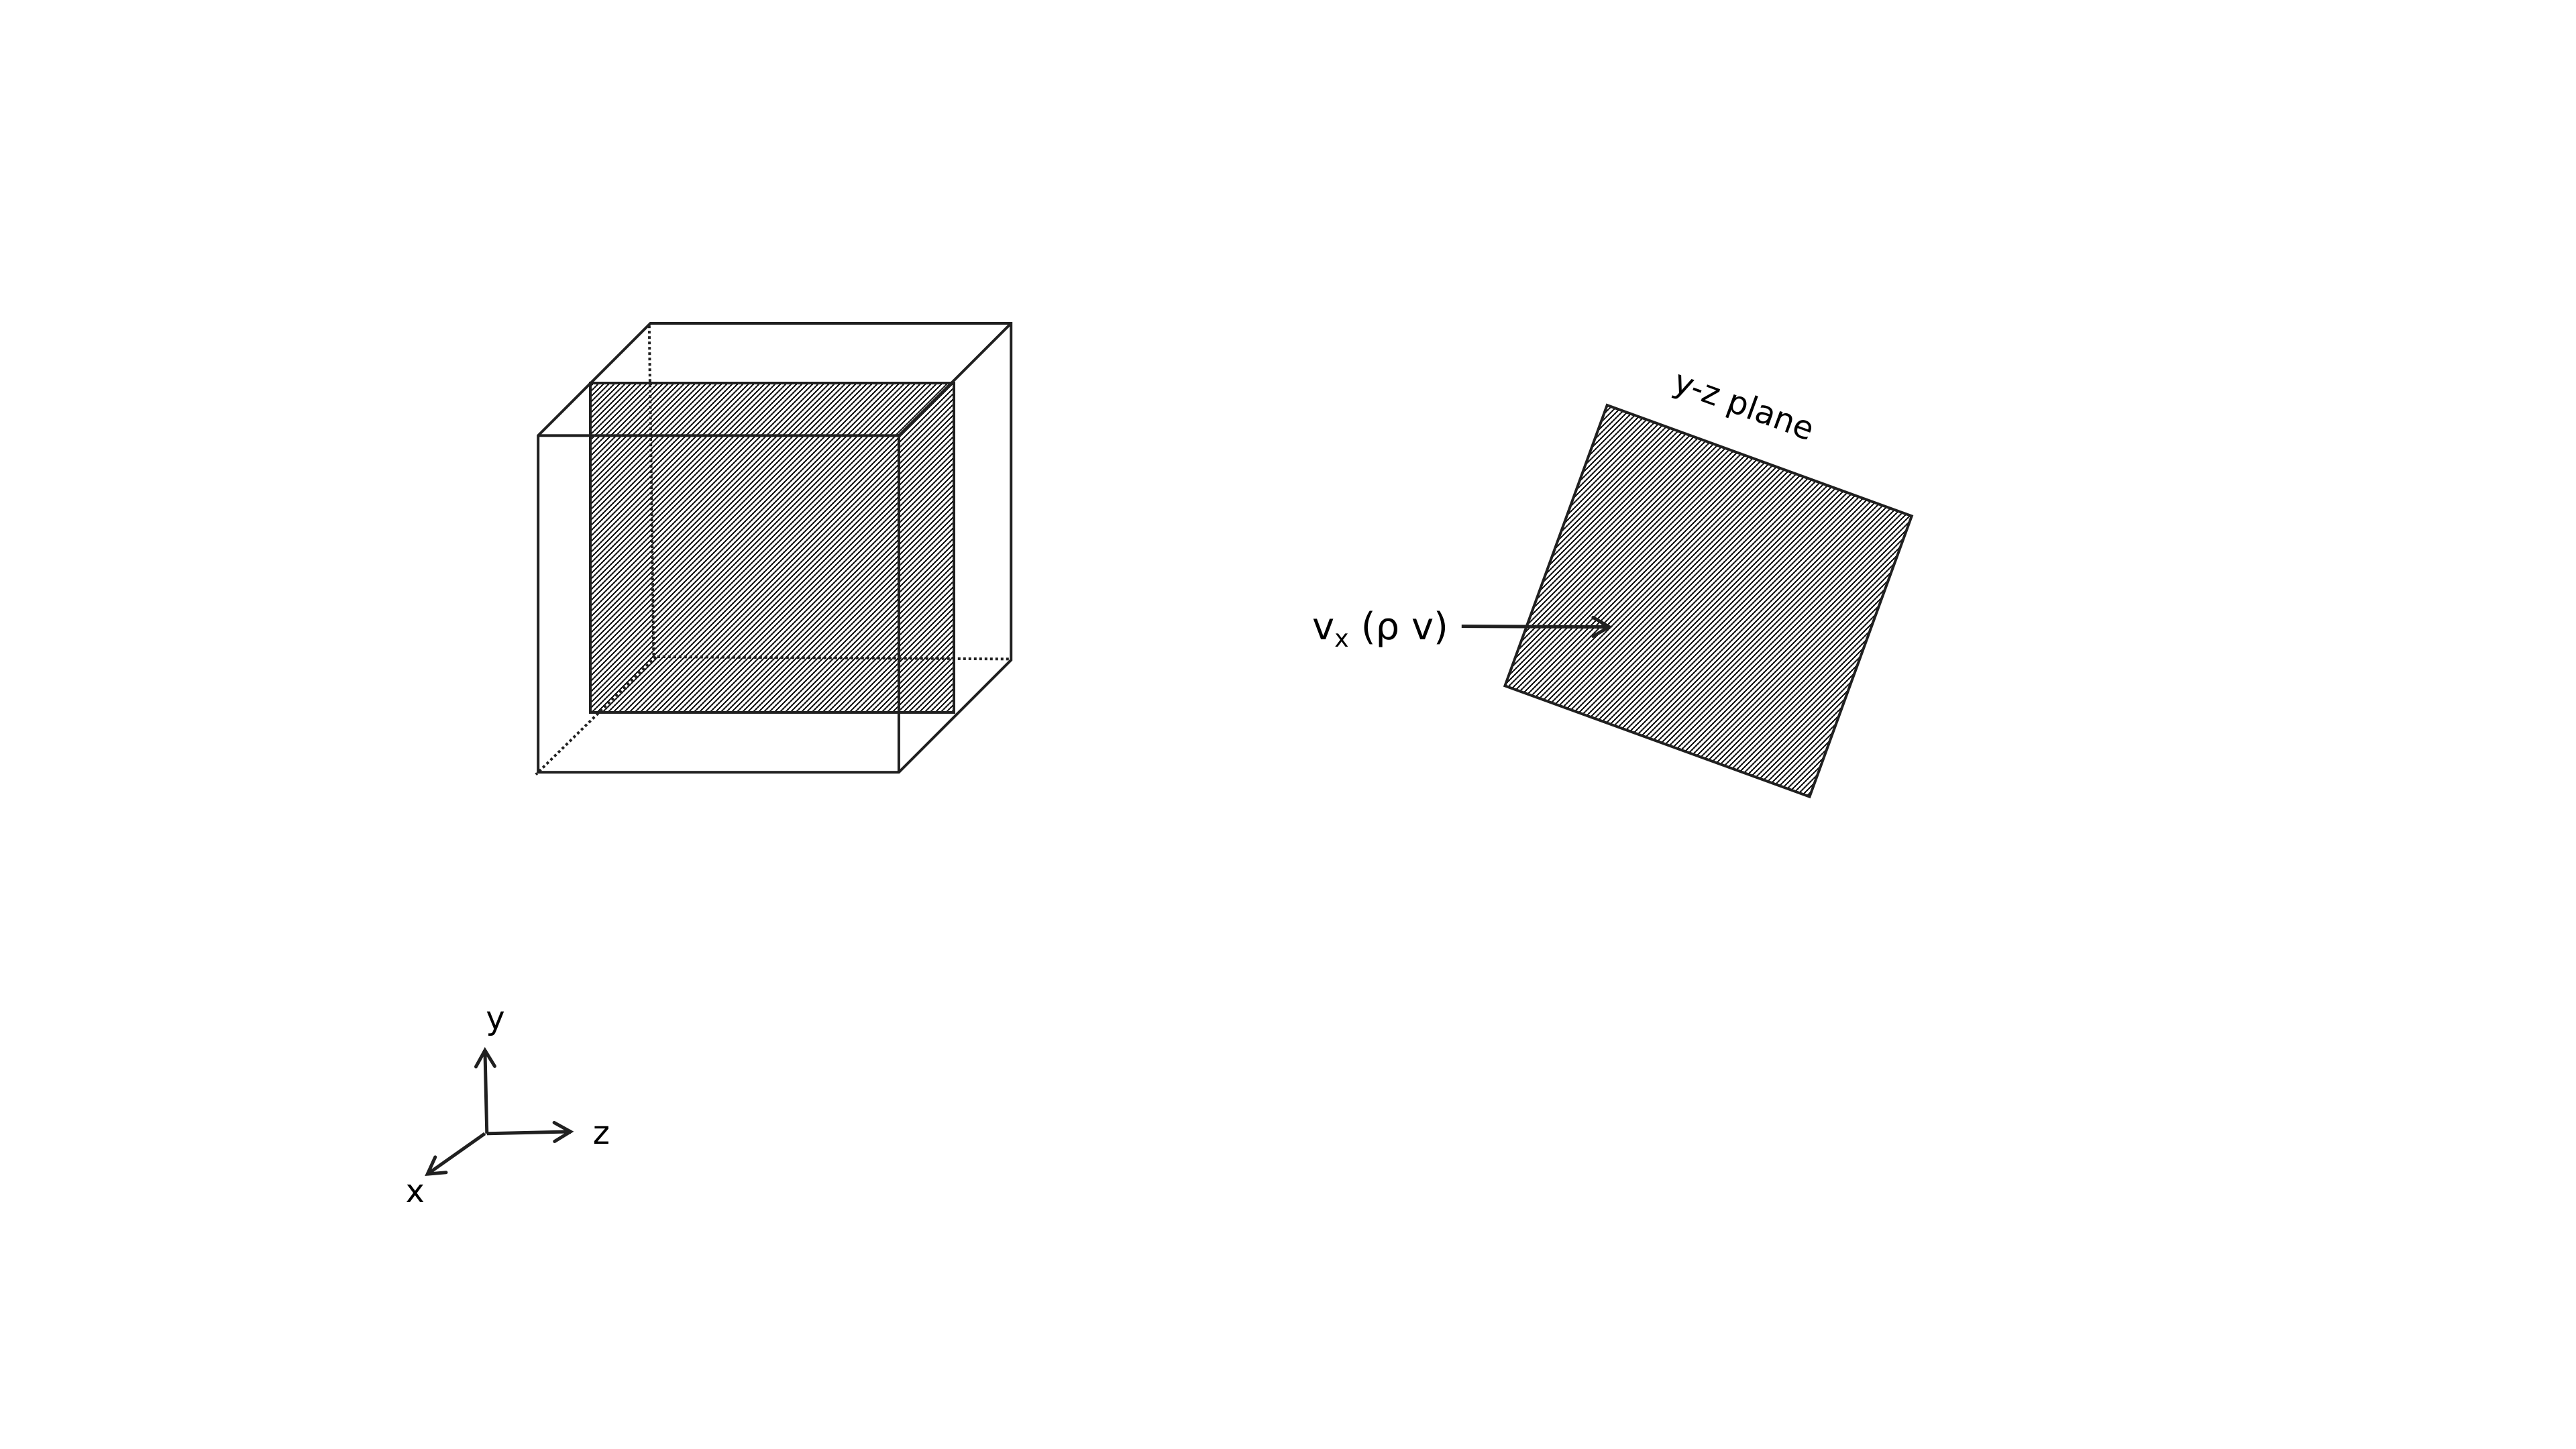
\includegraphics[scale=0.05]{figure2_02}
    \caption{Convective Momentum Transport}
\end{figure}

In figure 3, we see the same fluid element again, but this time let us only consider the convective terms. The volume rate of fluid flow across the shaded area is $v_{x}$. And it carries a momentum vector \textbf{$\rho$ v} (here we look at momentum per unit volume). Hence the momentum flux is simply $v_{x} \rho$ \textbf{v}. This quantity is the convective momentum flux across a plane perpendicular to the x-axis.

The tensor for convective momentum transport can be represented as $\rho$ \textbf{v v}. As in the case of molecular momentum flux tensor, this is also a 9-component tensor. 


\subsubsection*{Combined Momentum Flux}

To denote the total momentum flux experienced by a fluid in various directions, we use the tensor $\phi$. It is the sum of molecular and convective momentum fluxes.

\begin{empheq}[box=\fbox]{align}
    \phi = \pi + \rho \textbf{v v}
\end{empheq}

Consider some example components of this tensor:

$$\phi_{zz} = P + \tau_{zz} + \rho v_{z} v_{z}$$

$$\phi_{xy} = \tau_{xy} + \rho v_{x} v_{y}$$



\section*{Questions}

\begin{enumerate}
    \item Consider a set of vectors {\textbf{$v_{i}$}}, where all the vectors are orthogonal (perpendicular) to each other. We want to develop a terse notation to show this orthogonality. Which of these are suitable?

        (a) $v_{i} \cdot v_{j} = |v|^{2}$

        (b) $v_{i} \cdot v_{j} = |v|^{2} \delta_{ij}$

        (c) $v_{i} - v_{j} = (\delta_{x} - \delta_{y})(|v_{i}| - |v_{j}|)$ 

        (d) $v_{i} + v_{j} = (\delta_{x} + \delta_{y})(|v_{i}| + |v_{j}|)$

    \item Two infinite parallel plates, separated by 1m have a viscous static fluid of viscosity 1 cP between them. The top plate is translated to the left with a velocity of 5 $m s^{-1}$ and the bottom plate is translated to the right by 6 $m s^{-1}$. After reaching steady-state, what is the velocity of a fluid element half-way between the plates? Is that fluid element moving to the right or left?

    \item A boat with sophisticated measurement machinery is going around a lake on a windy day and measuring stresses. The velocity of the lakewater at a point (x, y) is given by $v_{x}(x, y), v_{y}(x, y)$, where $v_{x}(x, y) = A e^{-(x+y)}$, $v_{y}(x,y) = B \frac{x + y}{xy}$ Write the components of the viscous stress tensor for this system. 

    \item Verify that the per-volume momentum $\rho$ \textbf{v} when multiplied by velocity \textbf{v} does in fact give a momentum flux quantity.

\end{enumerate}

